\section{Kezdetek}

Első lépésként tanulmányoztam egy hasonló terméket, amely hasonlóan működik, 
viszont kevesebb funkcionalitással. Ebből megismerve a működési elvét és ezt fejlesztve 
terveztem meg a teszteremet. Legfontosabb része a teszternek egy mikrovezérlő, 
amely a rendszer magját adja, erre a célra egy Raspberry Pi Pico-t \cite{RaspberryPico} 
választottam, a nagyszámú GPIO-ja miatt, nagy teljesítménye miatt és nagy sebességű 
beépített hardveres kommunikációs protokollokkal (legfőképpen SPI \cite{SPIprotokol}). 
Ezután egy kijelző következett, amelyeken a teszter ki tudja jelezni az adatokat az adott 
komponensről. Erre a célra egy ILI9341 \cite{ILI9341Datasheet} kijelzőt használtam, ez 
egy 2.2” méretű színes TFT kijelző, és erre íródnak ki az adatok a felhasználó fele. 
Ezen kívül van 2 LED, amely a rendszer státuszát jelzi egyszerű színkódokkal. A teszteléshez 
szükséges áramkört a DAC segítségével történik és a mikrovezérlő csak a feszültség 
értékeket nézi, erre a célra egy DAC8565 \cite{DAC} DAC-ot használtam amely szintén 
SPI-on keresztül kommunikál a mikrovezérlővel. Ennek a 3 kimenete egy-egy 3 kimenetes 
analóg kapcsolón\cite{AnalogSwitch} keresztül különböző ellenállásokra kapcsolódnak a nagyobb precizitás 
elérése érdekében és az esetleges rövidzár esetén is az áramerősség biztonságos szinten 
tartásáért, minden esetben a létrehozott áramkörön lesz egy ellenállás, ami az 
áramerősséget limitálja, hogy esetlegesen ne tegye tönkre a tesztelés alatt levő 
alkatrészt. Miközben a mikrovezérlőnek 3 ADC (analog-digital converter) portja közvetlen 
rá van csatolva egy lábra ahová majd a tesztelni kívánt komponens kerül. A rendszernek 
van egy külső referencia feszültsége, ami egy stabil 3.3V-ot biztosít az ADC referenciaként 
és DAC referenciának.

\section{A rendszer tervezéséhez szükséges eszközök}

A rendszer tervezése egy Linux alapú számítógépen történt, de Windowson is hasonlóan
megoldható, mivel a használt programok mindkét operációs rendszer alatt futtathatóak,
lehetséges, hogy MAC alatt is hasonló, viszont azzal nincs tapasztalatom, így az nem biztos.

A rendszer áramkör terve a EasyEDA program segítségével történt, ez akár böngészőm keresztül is
használható. Nagy méretű adatbázisában legtöbb IC lábkiosztása megtalálható, így a 
tervrajz terverésekor méretarányos és megnevezett lábak sokat segítenek a vezetékek
bekötése során. Ezen kívűl ingyenesen használható, miközben kielégítő szolgáltatásokat nyújt.

A mikrovezérlő szoftver tervezéséhez szükség van egy könyvtárcsomagra amely szükséges
a mikrovezérlő programozásához. Ezt a részt Linux alatt használtam, ezen leírás alapján
\cite{PicoInstallLinux}, ez alapján lehet teleíteni a könyvtárcsomagot, amelyel C/C++ programozási
nyelvvel lehet programozni a rendszert, lehetséges micropython alatt is, viszont ezzel kevesebb
dokomentáció található, komplexebb dolgokra meg szinte semmi. Micropython-al lehet egyszerű
dolgokra használni, viszont nem egy ilyen projektre.

A szoftver C++-ban íródott, mivel ki tudja használni a legtöbb általános könyvtárcsomagot
és az osztályokba szervezve könnyebben szét lehet választani a különböző alrészeket. A kód 
nagyon hasonló egy átlagos C++ kódhoz, csupán ott különbözik az átlagos számítógépre írt C++ kódtól 
amikor az alsó szintet vezérli, mint például GPIO, ADC és a szemafor, 2. processzor mag elindítása.

A projektet lehet parancssorból is építeni, viszont Visual Studio Code alatt van egy kiterjesztés
amivel egy gombnyomásra felépíti a projektet. A projekt sikeres építése után a "build" mappában megjelenik
egy fájl amit majd fel kell tölteni a mikrovezérlőre.

\section{A rendszer Blokk váza}

A rendszerher működéséhez szükséges egy 5V-os feszültség forrás, ez lehet egy általános USB
tápforrás, vagy lehetséges direkt 5V csatlakoztatása is. Az áramerősség alacsony, így nem közelíti
meg az 500mA-es áramerősség határt amit egy átlagos USB képes leadni. Külső akkumulátorról
is táplálható. Amennyiben egy számítógéphez, vagy egy olyan eszközhöz van csatolva ami képes 
a serial portot olvasni akkor a mérési eredményeket automatikusan elküldi azon keresztül a 
másik eszköz felé. 

A pontos részleteket az a következőkben lesznek leírva.

\begin{figure}[H]
    \centering
    \subfigure[A rendszer block váza]{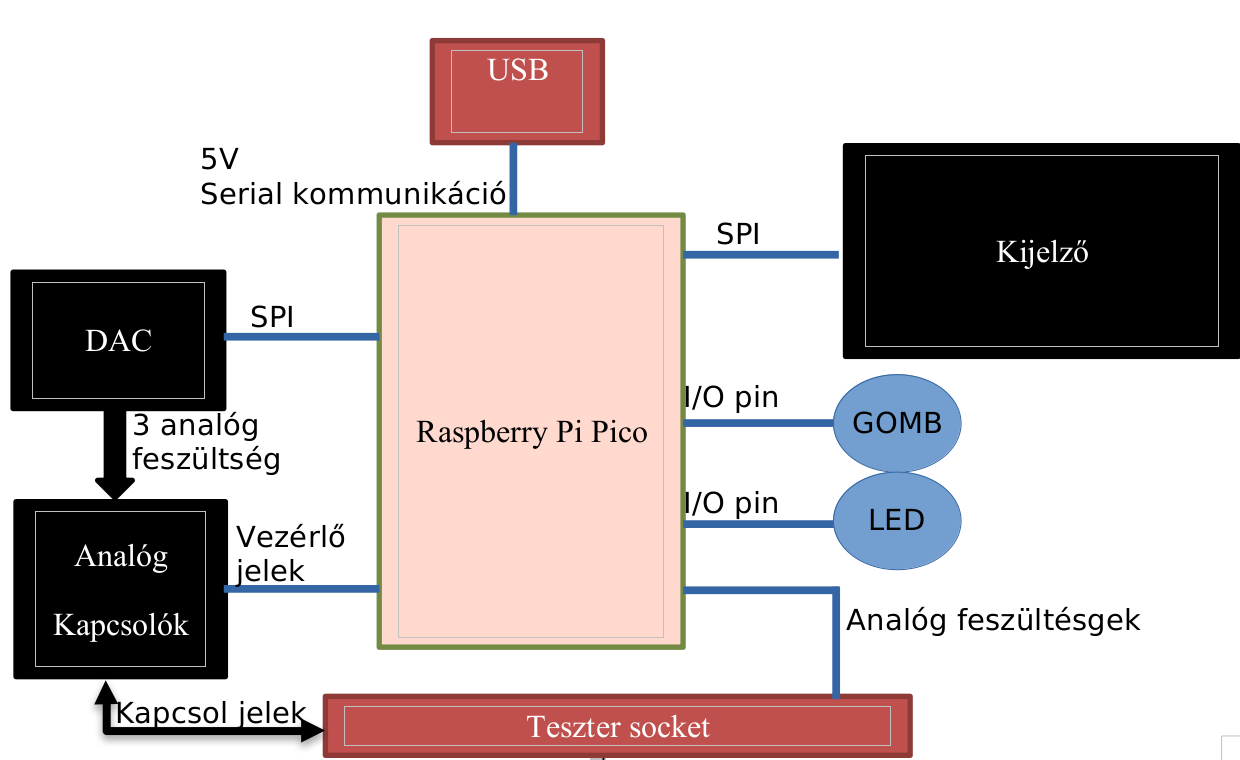
\includegraphics[scale=0.3]{figures/images/literature/blockDiagramm.png}}
    \caption{A rendszer block váza}
    \label{fig:blockDiagramm}
\end{figure}

\section{Fő komponensek részletes bemutatása}

A komponensek kiválasztásánál fontos szempont volt, hogy lehetőleg a legpontosabb 
eredményeket érje el, miközben lehetőleg egyszerű maradjon a rendszer és az áramfogyasztás 
is alacsony legyen és emellett hordozható legyen.

\subsection{Digital analog converter}
